\chapter{Approach}
\label{cha:Approach}
In the last section a few approaches have been outlined and discussed, that have successfully implemented methods regarding the creation of audios/music with a neural network approach. As seen, these have been mainly categorized in neural audio synthesis and neural audio style transfer. There current work has its main influence from the area neural audio synthesis, and can be categorized as such, as the methodology and workflow is strongly related to those works. Nevertheless regarding certain components, it has also its influence from the style transfer methods, despite not defining a specific content or style audio respective loss functions.

This chapter will therefore dive into the methodology and exact workflow of this works' solution, to the problem that also will help to derive the answers to the defined research questions. First an Overview/Motivation should provide the reader with the intended idea and an overview of the applied methods, to get a general understanding of the idea (see section \ref{sec:app_motivation}. Later on the single steps and components that are needed, in order reach the desired functionalities, are going to get described in detail, starting with the pre processing. Further on the ML-Model (neural network) will get described, as well as the step that is done to synthesize new sounds. Further on, the required steps for (re)generating a listenable audio as well as an description of the used dataset for training and also all experiments conducted later on (see chapter \ref{cha:Experiment}).

\section{Motivation}
\label{sec:app_motivation}
Like mentioned in the beginning of this thesis, this work aims to explore the possibilities of machine learning techniques such as neural networks, to apply in the audio domain for sound generation. This idea is mainly inspired by the idea of taking two distinct audio sources and mixing their characteristics in order to generate a new sound. As seen in the previous chapter, this idea is strongly related to the image domain, where the "synthesis" of a new pictures based on two source images, is commonly known as image style transfer (point \ref{sec:rw_imgstyletransfer}). This technique, of having a content image to be stylised with a certain style from another image, would mean for the application in the audio, to have a style sound to be transferred onto a content/target sound. Such approaches are specifically known as audio style transfer and can either be applied to single notes or also whole audio samples or songs. Having the principle of content and style this would mean, that of one sound the global structure and rhythmical components get preserved while imposing style (e.g. the timbre) on it to generate audios. The details to these approaches, have already been outlined in the previous chapter, when describing some existing work around this topic.

Neural audio synthesis is another method for neural sound generation, which does not apply the principles of style and content audio. In the previous chapter, some insights could be gained, how neural audio synthesis can look like, as well as how it can be achieved using different methods and neural networks. Most of those methods, were showing promising results, either concerning the auditory quality but also the possibilities that arise in experimenting and designing sounds. Those methods were using most of the time so called autoencoder networks, that can be used for dimensionality reduction of input data, as they have a so called "bottleneck" in the middle. \cite{hinton2006autoencoder} Because of this structure, the compressed data in this "bottleneck" represents essential features that either can be combined/interpolated or directly synthesized. To generate synthesized audio, the solutions described in section \ref{sec:rw_neural_audio_synthesis} used the "decompressing part" of the network to generate in order audio data. The exact workflow and methodologies for sound creation, have already been mentioned in the chapter related works (see chapter \ref{cha:related_works}, point \ref{sec:rw_neural_audio_synthesis}).

Out of those methodologies, when having the idea of using two instruments' characteristics, to generate audio, the approach of \textit{Engel et al.} \cite{Engel2017} using convolutional and WaveNet-style autoencoders yielded the most promising results. Promising especially in terms of output quality but also concerning its implementation/reproducability. With a provided interactive web application, the results of this solutions can be explored, whereas different sounds can be mixed based with a certain ratio. The results in the web application are based on the WaveNet-style autoencoder but according to the scientific article, the convolutional (baseline) also provides strong results. Implementing an approach with a WaveNet-style network would also go beyond the scope, not least also the computational costs would be too high. As also some audio style transfer methods, especially the approach by \textit{Ramani et al.} \cite{Ramani2018}, are using convolutional autoencoders, this kind of network was chosen to be preferable, to be applied in this work/research.

\section{Overview}
\label{sec:app_overview}
Based on the motivation and existing approaches, this work aims to propose a system, that uses a convolutional autoencoder network, for the task of neural audio synthesis. This systems' goal is to take two distinct audio samples as input, wheras the significant features, of those get extracted and interpolated, to in order (re)generate a novel sound in the end. In figure \ref{fig:toolchain} the general workflow of the toolchain is depicted in order to get an understanding, how this system is built up. 

 \begin{figure}[htb!]
	\caption{Overview of the proposed solution}
	\label{fig:toolchain}
	\centering
	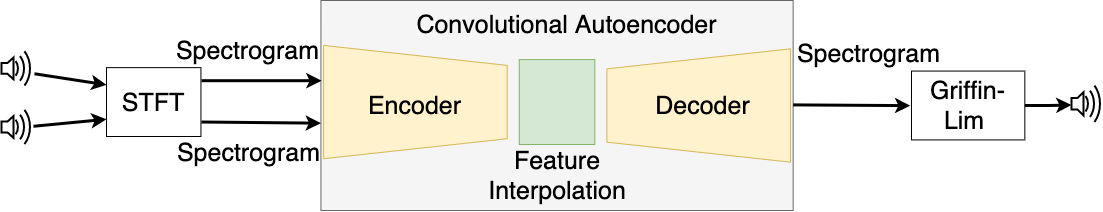
\includegraphics[width=\textwidth]{images/approach/Toolchain.png}
\end{figure}

Starting on the very left, two audios are taken and have to be brought into a suitable representation for this type of network. As audio is in its raw form a time-continuous signal and the input for convolutional networks are of a different shape (e.g. images) some pre-processing has to be done. In this case the short-term Fourier transform (STFT) is applied in order to generate a spectrogram, that shows the frequency spectra over the time. The frequency spectra contains on the one hand the magnitude (power) of the frequencies but also the phase information. For this purpose, only the magnitude data gets used, as its found to contain the most characteristic features of an audio. The ML-model (autoencoder) then takes the magnitude data as input, from which a compressed representation with the essential features gets generated with the lefthand (encoder) side. Having those features of two different audio samples, those get linearly interpolated, to generate one feature vector representing the "mixed" features of two instruments. This new vector, gets passed through the righthand (decoder) side of the network, which regenerates again spectral magnitude data of the same dimension as the input. In order to obtain a "playable" audio sound, it gets transformed back into time-domain with the Griffin-Lim algorithm \cite{Griffin1984} for phase estimation or the inverse short-term Fourier transform (ISTFT). The latter will be applied if there was no interpolation in the embedded space, as the phase information can be reused. Corresponding terminologies as well as a detailed insight into each step and its functionalities are given down below in the following points.

\section{Pre-processing}
\label{sec:app_pre-processing}
Pre-processing is the task of preparing raw data for a specific purpose. Moreover it is an important component of machine learning techniques such as for training neural networks. Deciding which pre-processing technique(s) to use on the one hand depends heavily on the type of ML-problem that has to be solved or even the training method that is chosen, but of course also on the type of data itself. As written before, for this work a neural network consisting of convolutional layers, has been chosen to be applied to the problem of neural audio synthesis. As convolutional neural networks are known for image processing tasks, they also can be applied for audio data, which has already been outlined in recent works in this field (see chapter \ref{cha:related_works}). In contrast to image data which most of the time has a 3D shape (width x length x RGB-colors), a raw audio has a different structure in its data representation, as it is a time-continuous signal (1D-shape). To in order bring the audio data in a similar shape, it has to undergo some pre-processing steps. Some representations of audio that have a image-like shape and can be used for deep learning tasks, include e.g. log-magnitude spectrograms or Mel-spectrograms but also Chromagrams and Constant-Q Transform (as stated by \cite{choi2018tutorial}). Taking the methods of recent works concerning neural audio synthesis into account, this work chooses to use the first two representation whereas in the experimental part of this work, they are going to be compared concerning the synthesis task and the performance of the neural network. <Maybe mention that spectrograms are found beneficial as they contain most essential data>

As the practical part of the project to this thesis is implemented in python, whereas a special library was used for the pre-processing part. For this part the library librosa \cite{brian_mcfee_2022_6097378} was being used, as it provides practical functions for audio processing, that were considered as useful for this work. Special to mention here are the functionalities as calculating spectrograms (STFT) but also transforming spectral data back into time domain to generate playable audio data (ISTFT, Griffin-Lim).


\subsection{Spectrograms and STFT}
Spectrograms represent a 2D-representation of an time-continuous signal, which essentially shows the presence of certain frequency bands over time. Like previously said, there exist different forms of spectrograms e.G. log-magnitude and log-mel spectrograms. Especially speaking of the log-magnitude spectrogram whose calculation is based on the short-time Fourier transform (STFT) and thus on the Fourier transform. The Fourier transform, takes a frame of $N$ values of an (audio) signal and transforms it from the time domain into the frequency domain. Generally said, that the bigger the frame, the better is the frequency resolution. What this means in terms of calculating the spectrogram, will get outlined shortly. Whats also important to mention at this point is, that the result of the Fourier transform, consists of an array of $N$ complex numbers, which are mirrored in the middle. Every complex number in this array stands for a so called frequency bin in the signal. The real part of these numbers would represent the power/magnitude of this "bin" and the imaginary part gives information about the phase. Coming back to the frequency resolution, this for example means that when taking a one-second signal with a sampling rate $SR$ and performing the Fourier transform with length $N=SR$ on it this would yield an array of $N$ values. The first value in the result depicts the signal's offset whereas all values from 1 to N/2 are the frequency bins with a resolution of 1Hz per bin. This means that each of this bin shows the magnitude and also phase of each frequency from 1 to N/2 Hz. The ongoing values in the result, show the same values except they are mirrored, as they depict the negative frequencies. (maybe some more explanation or citation) Because of this behaviour, the second part can be omitted for further use. Now these values just show the frequency spectra of one time frame and do not incorporate more information about the change. To overcome this shortcomming, the Fourier transform can get applied to a series of frames of the signal in order to obtain multiple frequency spectras over time that can be depicted as a spectrogram.\\

The calculation of multiple frequency spectras over time is the so called short-time Fourier transform. This form of calculation is widely used for pre-processing of audio data for ML-Tasks (for example see chapter \ref{cha:related_works}). When applying this transform, a few parameters have to be considered, as those influence the result but also the quality for the later workflow. One of the the most important parameters is \texttt{n\_fft} as it specifies the actual length of the signal-frame, on which the FFT (fast Fourier transform) gets applied to. This parameter therefore influences therefore, the frequency- but also time-resolution in the final spectrogram. To be mentioned regarding the official Librosa documentation, this should be a value of a power of two, as it speeds up the computation of the FFT behind. Another important parameter would be the \texttt{hop\_length}, which defines how much audio values are between the beginning of the first and the following frame. This means that when defining this parameter to \texttt{n\_fft/2} this would yield in a 50\% overlap of the following frame. Modifying this parameter, would mean to either increase or decrease the overlap and also the amount of time columns as more overlapping frames occur. The overlap of the frames is also coherent with the chosen window function for the STFT. As every time when the FFT gets applied to a frame, this one gets multiplied with a so called "window". Multiplying a signal frame with a window has to be done, as the FFT assumes, that the transformed signal is periodic (repeating itself infinitely). \cite{heinzel2002spectrum} This gets problematic when the input signal does contain frequencies that may not directly fall into a frequency bin, due to the FFT's frequency resolution. Due to the assumed cyclic continuation the Fourier transform will 'think' that there is a discontinuity and will spread therefore the power over all the spectrum. There exist multiple window functions such as "Hann", "Hamming", "Blackman", etc. which start at (almost) zero, rises to a maximum in the middle but falls again to (almost) zero at the end (symmetric). Multiplying the signal frame with such a window function helps to overcome this issue as it removes the discontinuity. On which window to chose, depends on the usecase of the application, whereas throughout this work a "Hann"-window was chosen all the time. Coming back to the relation with the window overlap, if no overlap would be used a lot of information of the signal would get lost. This is because when multiplying the signal frames with the window functions, this would bring very little or zero values at the beginning and end of the frame. \cite{heinzel2002spectrum} When having overlapping frames this issue would get corrected. Important here is again the amount of overlap as this is dependent on the window and its wideness. Using the "Hann"-window a common value for the overlap would be 50\% which was also considered throughout this work. This value is also beneficial later on, when performing the inverse transformation, back into time domain, but more on that in section \ref{sec:app_post_processing}. Beside of these parameters some more exist, for example for specifying the padding of the signal whereas in this work a constant padding on both sides of the signal has been used, which is also the default setting.\\

Now having the knowledge of the STFT and its parameters, it can be applied onto a signal, to generate a spectrogram. For example by using an audio sample with a sample rate of 16 kHz and applying the STFT with a n\_fft value of 1024 and a hop-length of 512 this would result in a spectrogram with a frequency resolution of 15,625 Hz but time resolution of 64 ms. As explained before, the values of the result, consist of complex numbers which contain the magnitude but also the phase at each frequency bin. By setting this result absolute, or calling the function \texttt{librosa.magphase(spectrogramm)} the real magnitude data can be obtained, whereas the latter also retrieves phase information in a separate vector. The magnitude here displays the energy values of the spectrogram, whereas for further processing and also to be better displayable those get converted into a dB-scale. \footnote{normally the magnitude would need to get squared to obtain the power, but in this case magnitude without squaring was taken} As this function also takes a reference value that gets set to 0 dB, which in this case will be the maximum value of the magnitude spectrum. As for post-processing when converting the dB-scaled data back into energy, also a reference value is needed, this one gets preserved, in order to get the same scaling as in the original input. Finally when having the log-mag spectrograms in dB, those were considered for the training of the neural network afterwards. An example of a log-mag spectrogram can be seen in figure \ref{fig:spectrogram}. As also the phase information also was obtained when calculating the magnitude data, this one was also preserved next to the energy reference value for the recreation of signals, as it is needed there (this will mainly affect the recreation of single samples, without interpolation in embedded space, but more on that later on).


 \begin{figure}[htb!]
	\caption{STFT log-mag spectrogram of a guitar note}
	\label{fig:spectrogram}
	\centering
	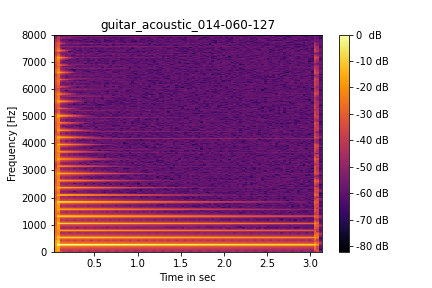
\includegraphics[width=0.8\textwidth]{images/approach/guitar_acoustic_014-060-127.png}
\end{figure}

This section describes the general workflow of the pre-processing from taking a signal and converting it into a spectral representation. This workflow is a basis on which different experiments with different parameterization (size of n\_fft, etc. ) of the calculation of the spectrograms but also with additional steps (log-mel scale, additional framing, etc.) are being made. Those steps will get mentioned later on in chapter \ref{cha:Experiment} when describing the experimental part of the thesis.

\section{ML-Model}
\label{sec:app_model}
The main or core component of every machine learning project is of course the model itself, as it achieves the main task of prediction or inference to a given problem. Those models exist as different technologies that perform regression tasks or even classification tasks. Dependent on the usecase, but also the kind of data that is present, different models are better suited or not. To count technologies, there exist the KNN-Algorithm, Decision-Trees, Random Forests, Support-Vector-Machines (SVM) but also neural networks which can be applied in a variety of usecases. Especially the latter, the neural networks, are able to achieve a variety of different tasks, as they are highly adaptive regarding their topology, used layers, but also the size and shape. Those variety of different tasks spread across different domains, so also for images and audio. 

\subsection{Neural Networks - Introduction}
Generally said a neueral network can be seen as a graph of connected nodes  with numeric values that can achieve transformations between patterns using message-passing algorithms. \cite{Jordan1996neuralnets} Those nodes are commonly structered in layers, where there especially exist certain nodes or even layers that are seen as input nodes/layers and some as output nodes/layers. Between the input and the output there can also exist some so called hidden layers, expanding the depth of the network. The links between the nodes, that get also called neurons, are connected via links, that are parameterized with weights, that get optimized using learning algorithms. Each neuron receives its weighted input (activities) of its connected predecessors, which get converted into a single output that gets broadcast to all its connected successors. \cite{hinton1992neural} The latter involves a so called input-output function which is also commonly known as activation function (e.G. ReLU, Sigmoid ...). Also important to know, is that the weights on the connections define how much this value influences the input of the connected node. 
When a neural network gets trained to a specific problem (e.g. classifying certain images), using predetermined training data, the output of the neural network gets compared with the desired one, resulting in a certain error. To minimize this error, the weights in the network get adapted by back-propagating the error through all the layers, to the beginning. On this way it changes the influence of certain connections and therefore the overall outcome. This procedure gets repeated on all training data over several iterations, until the error gets low to produce the desired output. Depending on the problem to solve / what's the desired output, neural networks can be trained using labeled data (supervised) but also just by minimizing a cost function (unsupervised).\cite{oshea2015introductionConv} More on that 

\subsection{}

<convergence?, learning rate, 

\section{Post Processing}
\label{sec:app_post_processing}

\section{Interpolation in latent space}
\label{sec:app_interpolation}

\section{Dataset}
\label{sec:app_dataset}